% This is samplepaper.tex, a sample chapter demonstrating the
% LLNCS macro package for Springer Computer Science proceedings;
% Version 2.25 of 2026/09/03
%
\documentclass[runningheads]{llncs}
%
\usepackage[T1]{fontenc}
% T1 fonts will be used to generate the final print and online PDFs,
% so please use T1 fonts in your manuscript whenever possible.
% Other font encondings may result in incorrect characters.
%

\usepackage{newtxtext}       % 
\usepackage[varvw]{newtxmath}       % selects Times Roman as basic font


\usepackage{graphicx}
\usepackage{amssymb}
% Used for displaying a sample figure. If possible, figure files should
% be included in EPS format.
%
% If you use the hyperref package, please uncomment the following two lines
% to display URLs in blue roman font according to Springer's eBook style:
%\usepackage{color}
%\renewcommand\UrlFont{\color{blue}\rmfamily}
%\urlstyle{rm}
%
\begin{document}
%
\title{Succinct Graph Representations}
%
%\titlerunning{Abbreviated paper title}
% If the paper title is too long for the running head, you can set
% an abbreviated paper title here
%
\author{Jose,Nimisha Ann \inst{1} \and
Jose,Gilmy\inst{1}\and
Yevge,Aman Pravin\inst{1}}
%
%\authorrunning{F. Author et al.}
% First names are abbreviated in the running head.
% If there are more than two authors, 'et al.' is used.
%
\institute{Trier University, Trier ,Germany }
%
\maketitle              % typeset the header of the contribution
%
%\begin{abstract}
%The abstract should briefly summarize the contents of the paper in
%150--250 words.

%\keywords{First keyword  \and Second keyword \and Another keyword.}
%\end{abstract}
%
%
%
\section{Introduction}
% ==========================================================================
\section{Preliminaries}
\label{sec:preliminaries}
% ==========================================================================

$\mathbf{N}$ includes $0$,
$[n] = \{1, \dots, n\}$, $\mathbb{N}_{\ge n} = \{ k \in \mathbb{N} \mid k \ge n \}$, and
$\binom{X}{k}$ is the set of $k$-element subsets of $X$.

\subsection{Words and Languages}


\section{Propositions}
%\subsection{A Subsection Sample}
%Please note that the first paragraph of a section or subsection is
%not indented. The first paragraph that follows a table, figure,
%equation etc. does not need an indent, either.

%Subsequent paragraphs, however, are indented.

%\subsubsection{Definition 1(Graph)} A graph $G$ is defined as an ordered pair $(V,E)$  ; where $V$ is the set of vertices or nodes, and $E$ is the set of edges.



%\paragraph{Sample Heading (Fourth Level)}
%The contribution should contain no more than four levels of
%headings. Table~\ref{tab1} gives a summary of all heading levels.

%\begin{table}
%\caption{Table captions should be placed above the
%tables.}\label{tab1}
%\begin{tabular}{|l|l|l|}
%\hline
%Heading level &  Example & Font size and style\\
%\hline
%Title (centered) &  {\Large\bfseries Lecture Notes} & 14 point, bold\\
%1st-level heading &  {\large\bfseries 1 Introduction} & 12 point, bold\\
%2nd-level heading & {\bfseries 2.1 Printing Area} & 10 point, bold\\
%3rd-level heading & {\bfseries Run-in Heading in Bold.} Text follows & 10 point, bold\\
%4th-level heading & {\itshape Lowest Level Heading.} Text follows & 10 point, italic\\
%\hline
%\end{tabular}
%\end{table}


%\noindent Displayed equations are centered and set on a separate
%line.
%\begin{equation}
%x + y = z
%\end{equation}
%Please try to avoid rasterized images for line-art diagrams and
%schemas. Whenever possible, use vector graphics instead (see
%Fig.~\ref{fig1}).

%\begin{figure}
%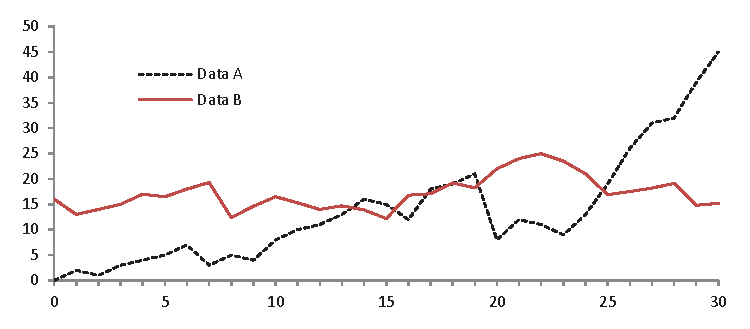
\includegraphics[width=\textwidth]{fig1.eps}
%\Description{In LaTeX you may insert your alternative texts into your manuscript using the \verb|\Description| command in a \verb|figure| environment}
%\caption{A figure caption is always placed below the illustration.
%Please note that short captions are centered, while long ones are
%justified by the macro package automatically.} \label{fig1}
%\end{figure}

\begin{proposition}
The shortest possible word $w$ that agrees with $C_4$ on $L_{\neg 1^{3}}$ has length $8$ . One such word is $w = 22132433$.
\end{proposition}



%
% the environments 'definition', 'lemma', 'proposition', 'corollary',
% 'remark', and 'example' are defined in the LLNCS documentclass as well.
%
\begin{proof}
Let the smallest possible word $w$ be $w = 22132433$ and $|w| = 8$. The alphabet $\Sigma = \{1,2,3,4\}.$ The word $w$ contains the elements of $\Sigma$ at least once, i.e., every vertex occurs. Now the pair $\{u,v\}$ is a non-edge iff $h_{\{u,v\}}(w)$ contains $000$ or $111$. This implies that one of the two letters occurs at least $3$ times in a row in the projection, which in turn implies that it occurs at least $3$ times in $w$.Also, the non-edges of $C_4$ are $\{1,3\}$ and $\{2,4\}$, and they are disjoint. One letter from $\{1,3\}$ and one letter from $\{2,4\}$ must each occur at least $3$ times, and the remaining two letters must each occur at least once. Therefore, $|w| \geq 3+1+3+1 = 8$, i.e., $|w| = 8$ is optimal.
\end{proof}

\begin{proposition}
The shortest possible word $w$ that agrees with $C_4$ on $L_{1112}$ has length $9$. One such word is $w = 223121413$.
\end{proposition}

\begin{proof}
Let the smallest possible word $w$ be $w = 223121413 $ and $|w| = 9$.The alphabet $\Sigma = \{1,2,3,4\}.$ The word $w$ contains the elements of $\Sigma$ at least once, i.e., every vertex occurs. Now the pair $\{u,v\}$ is a non-edge iff $h_{\{u,v\}}(w)$ contains $0001$ or $1110$. This implies that one of the two letters occurs at least $3$ times and the other letter occurs at least once  in a row in the projection, which in turn implies that together $u$ and $v$ occur  at least $4$ times in $w$.Also, the non-edges of $C_4$ are $\{1,3\}$ and $\{2,4\}$, and they are disjoint.  Therefore, $|w| \geq 4+4 = 8$.
Now, assume  $|w| = 8$ .
Then $\{1,3\}$ and $\{2,4\}$ each has exactly $4$ occurances.So each non-edge contributes $(3,1)$ to the occurrence counts of $u$ and $v$. Assume that $1$ and $2$ occur $3$ times each, and that $3$ and $4$ occur once each. Let $P_1$ denote the position of the last occurrence of $1$ and $P_2$ the position of the last occurrence of $2$. Let $P_3$ and $P_4$ denote the positions of the letters $3$ and $4$, respectively.So each non-edge corresponds to the counts $(3,1)$: the letter occurring three times, $u$, is mapped to $0$, and the letter occurring once, $v$, is mapped to $1$, i.e., $u \to 0$ and $v \to 1$. The forbidden factor is then $uuuv$. Hence the pair $\{u,v\}$ is a non-edge if and only if $v$ comes after all three occurrences of $u$. Equivalently, the pair is an edge if and only if $v$ comes before the last occurrence of $u$.

Therefore we obtain the following inequalities:
\begin{align}
\{1,3\} \text{ is a non-edge:} \quad & P_3 > P_1, \label{ineq1}\\
\{2,4\} \text{ is a non-edge:} \quad & P_4 > P_2, \label{ineq2}\\
\{1,4\} \text{ is an edge:} \quad & P_4 < P_1, \label{ineq3}\\
\{2,3\} \text{ is an edge:} \quad & P_3 < P_2. \label{ineq4}
\end{align}
Combining \eqref{ineq1}--\eqref{ineq4}, we get
\[
P_1 < P_3 < P_2 < P_4 < P_1,
\]
which is a contradiction. Therefore $|w| = 8$ is not possible, so $|w| \geq 9$, and $|w| = 9$ is optimal.
\end{proof}

\begin{proposition}
The shortest possible word $w$ that agrees with $C_4$ on $L_{2-11}$ has length $12$. One such word is $w = 2124432321$.
\end{proposition}

\begin{proof}
    
\end{proof}

\begin{proposition}
The shortest possible word $w$ that agrees with $C_4$ on $L_{P}$ has length $6$. One such word is $w = 423142$.
\end{proposition}

\begin{proof}
Let the smallest possible word $w$ be $w = 423142 $ and $|w| = 6$. The alphabet $\Sigma = \{1,2,3,4\}.$ The word $w$ contains the elements of $\Sigma$ at least once, i.e., every vertex occurs. Now, for an edge  $\{u,v\}$, both letter appear in the projection.There is no palindrome of length $1$ that makes a pair an edge. Moreover, a palindrome of length $2$ consists of only one letter, either $u$ or $v$, which leads to the non-edge condition. Therefore, the projection $h_{\{u,v\}}(w)$ of an edge has length at least $3$. This implies that the two letters $u$ and $v$ occur at least $3$ times together in $w$. Hence one of the letters $u$ or $v$ occurs at least twice, and the other occurs at least once in $w$.The edges $\{1,2\}$ and $\{3,4\}$ are disjoint. Therefore, one letter from $\{1,2\}$ and one letter from $\{3,4\}$ occur at least twice, and the remaining two letters  each occur at least once. Therefore, $|w| \geq 2+1+2+1 = 6$, i.e., $|w| = 6$ is optimal.
\end{proof}
\begin{proposition}
    The shortest possible word $w$ that agrees with $C_4$ on $L_{C}$ has length $8$. One such word is $w = 23124134$.
\end{proposition}
\begin{proof}
    Let the smallest possible word $w$ be $w = 23124134 $ and $|w| = 8$. The alphabet $\Sigma = \{1,2,3,4\}.$ The word $w$ contains the elements of $\Sigma$ at least once, i.e., every vertex occurs. The pair  $\{u,v\}$ is an edge iff the projection $h_{\{u,v\}}(w)$ is a copy-word. Since every letter of the alphabet is a vertex, the projection $h_{\{u,v\}}(w)$ must have length at least $4$ for $\{u,v\}$ to be an edge, so each edge forces a count of at least $2$ on one of its letters. The edges of $C_4$ are $\{1,2\}$, $\{2,3\}$, $\{3,4\}$ and $\{4,1\}$. Hence every letter $1,2,3,4$ must occur at least twice in $w$. Therefore $|w| \geq 2 \cdot 4 = 8$, and $|w| = 8$ is optimal.
\end{proof}

\begin{proposition}
    The shortest possible word $w$ that agrees with $C_4$ on $L_{D}$ has length $8$. One such word is $w = 24342113$.
\end{proposition}

\begin{proposition}
    The shortest possible word $w$ that agrees with $C_4$ on $L_{L}$ has length $6$. One such word is $w = 131242$.
\end{proposition}
%For citations of references, we prefer the use of square brackets
%and consecutive numbers. Citations using labels or the author/year
%convention are also acceptable. The following bibliography provides
%a sample reference list with entries for journal
%articles~\cite{ref_article1}, an LNCS chapter~\cite{ref_lncs1}, a
%book~\cite{ref_book1}, proceedings without editors~\cite{ref_proc1},
%and a homepage~\cite{ref_url1}. Multiple citations are grouped
%\cite{ref_article1,ref_lncs1,ref_book1},
%\cite{ref_article1,ref_book1,ref_proc1,ref_url1}.

%\begin{credits}
%\subsubsection{\ackname} A bold run-in heading in small font size at the end of the paper is
%used for general acknowledgments, for example: This study was funded
%by X (grant number Y).

%\subsubsection{\discintname}
%It is now necessary to declare any competing interests or to specifically
%state that the authors have no competing interests. Please place the
%statement with a bold run-in heading in small font size beneath the
%(optional) acknowledgments\footnote{If EquinOCS, our proceedings submission
%system, is used, then the disclaimer can be provided directly in the system.},
%for example: The authors have no competing interests to declare that are
%relevant to the content of this article. Or: Author A has received research
%grants from Company W. Author B has received a speaker honorarium from
%Company X and owns stock in Company Y. Author C is a member of committee Z.
%\end{credits}

%
% ---- Bibliography ----
%
% BibTeX users should specify bibliography style 'splncs04'.
% References will then be sorted and formatted in the correct style.
%
% \bibliographystyle{splncs04}
% \bibliography{mybibliography}
%
%\begin{thebibliography}{8}
%\bibitem{ref_article1}
%Author, F.: Article title. Journal \textbf{2}(5), 99--110 (2016)

%\bibitem{ref_lncs1}
%Author, F., Author, S.: Title of a proceedings paper. In: Editor,
%F., Editor, S. (eds.) CONFERENCE 2016, LNCS, vol. 9999, pp. 1--13.
%Springer, Heidelberg (2016). \doi{10.10007/1234567890}

%\bibitem{ref_book1}
%Author, F., Author, S., Author, T.: Book title. 2nd edn. Publisher,
%Location (1999)

%\bibitem{ref_proc1}
%Author, A.-B.: Contribution title. In: 9th International Proceedings
%on Proceedings, pp. 1--2. Publisher, Location (2010)

%\bibitem{ref_url1}
%LNCS Homepage, \url{http://www.springer.com/lncs}, last accessed 2023/10/25
%\end{thebibliography}
\end{document}
